\documentclass[english]{tktltiki}
\usepackage[pdftex]{graphicx}
\usepackage{subfigure}
\usepackage{booktabs}
\usepackage{url}
\usepackage{amsthm,amssymb}
 \usepackage{amsmath}
 \usepackage{enumerate}
 
 \usepackage{chngcntr}
\counterwithin*{equation}{section}
\counterwithin*{equation}{subsection}

\begin{document}
\onehalfspacing

\title{Workshop 7}
\author{P�ter Ivanics}
\date{\today}

\maketitle

\section{Problems 1-4}
Note: the formulas are already written in with their negated forms in the scanned handwriting below.
	\begin{center}
		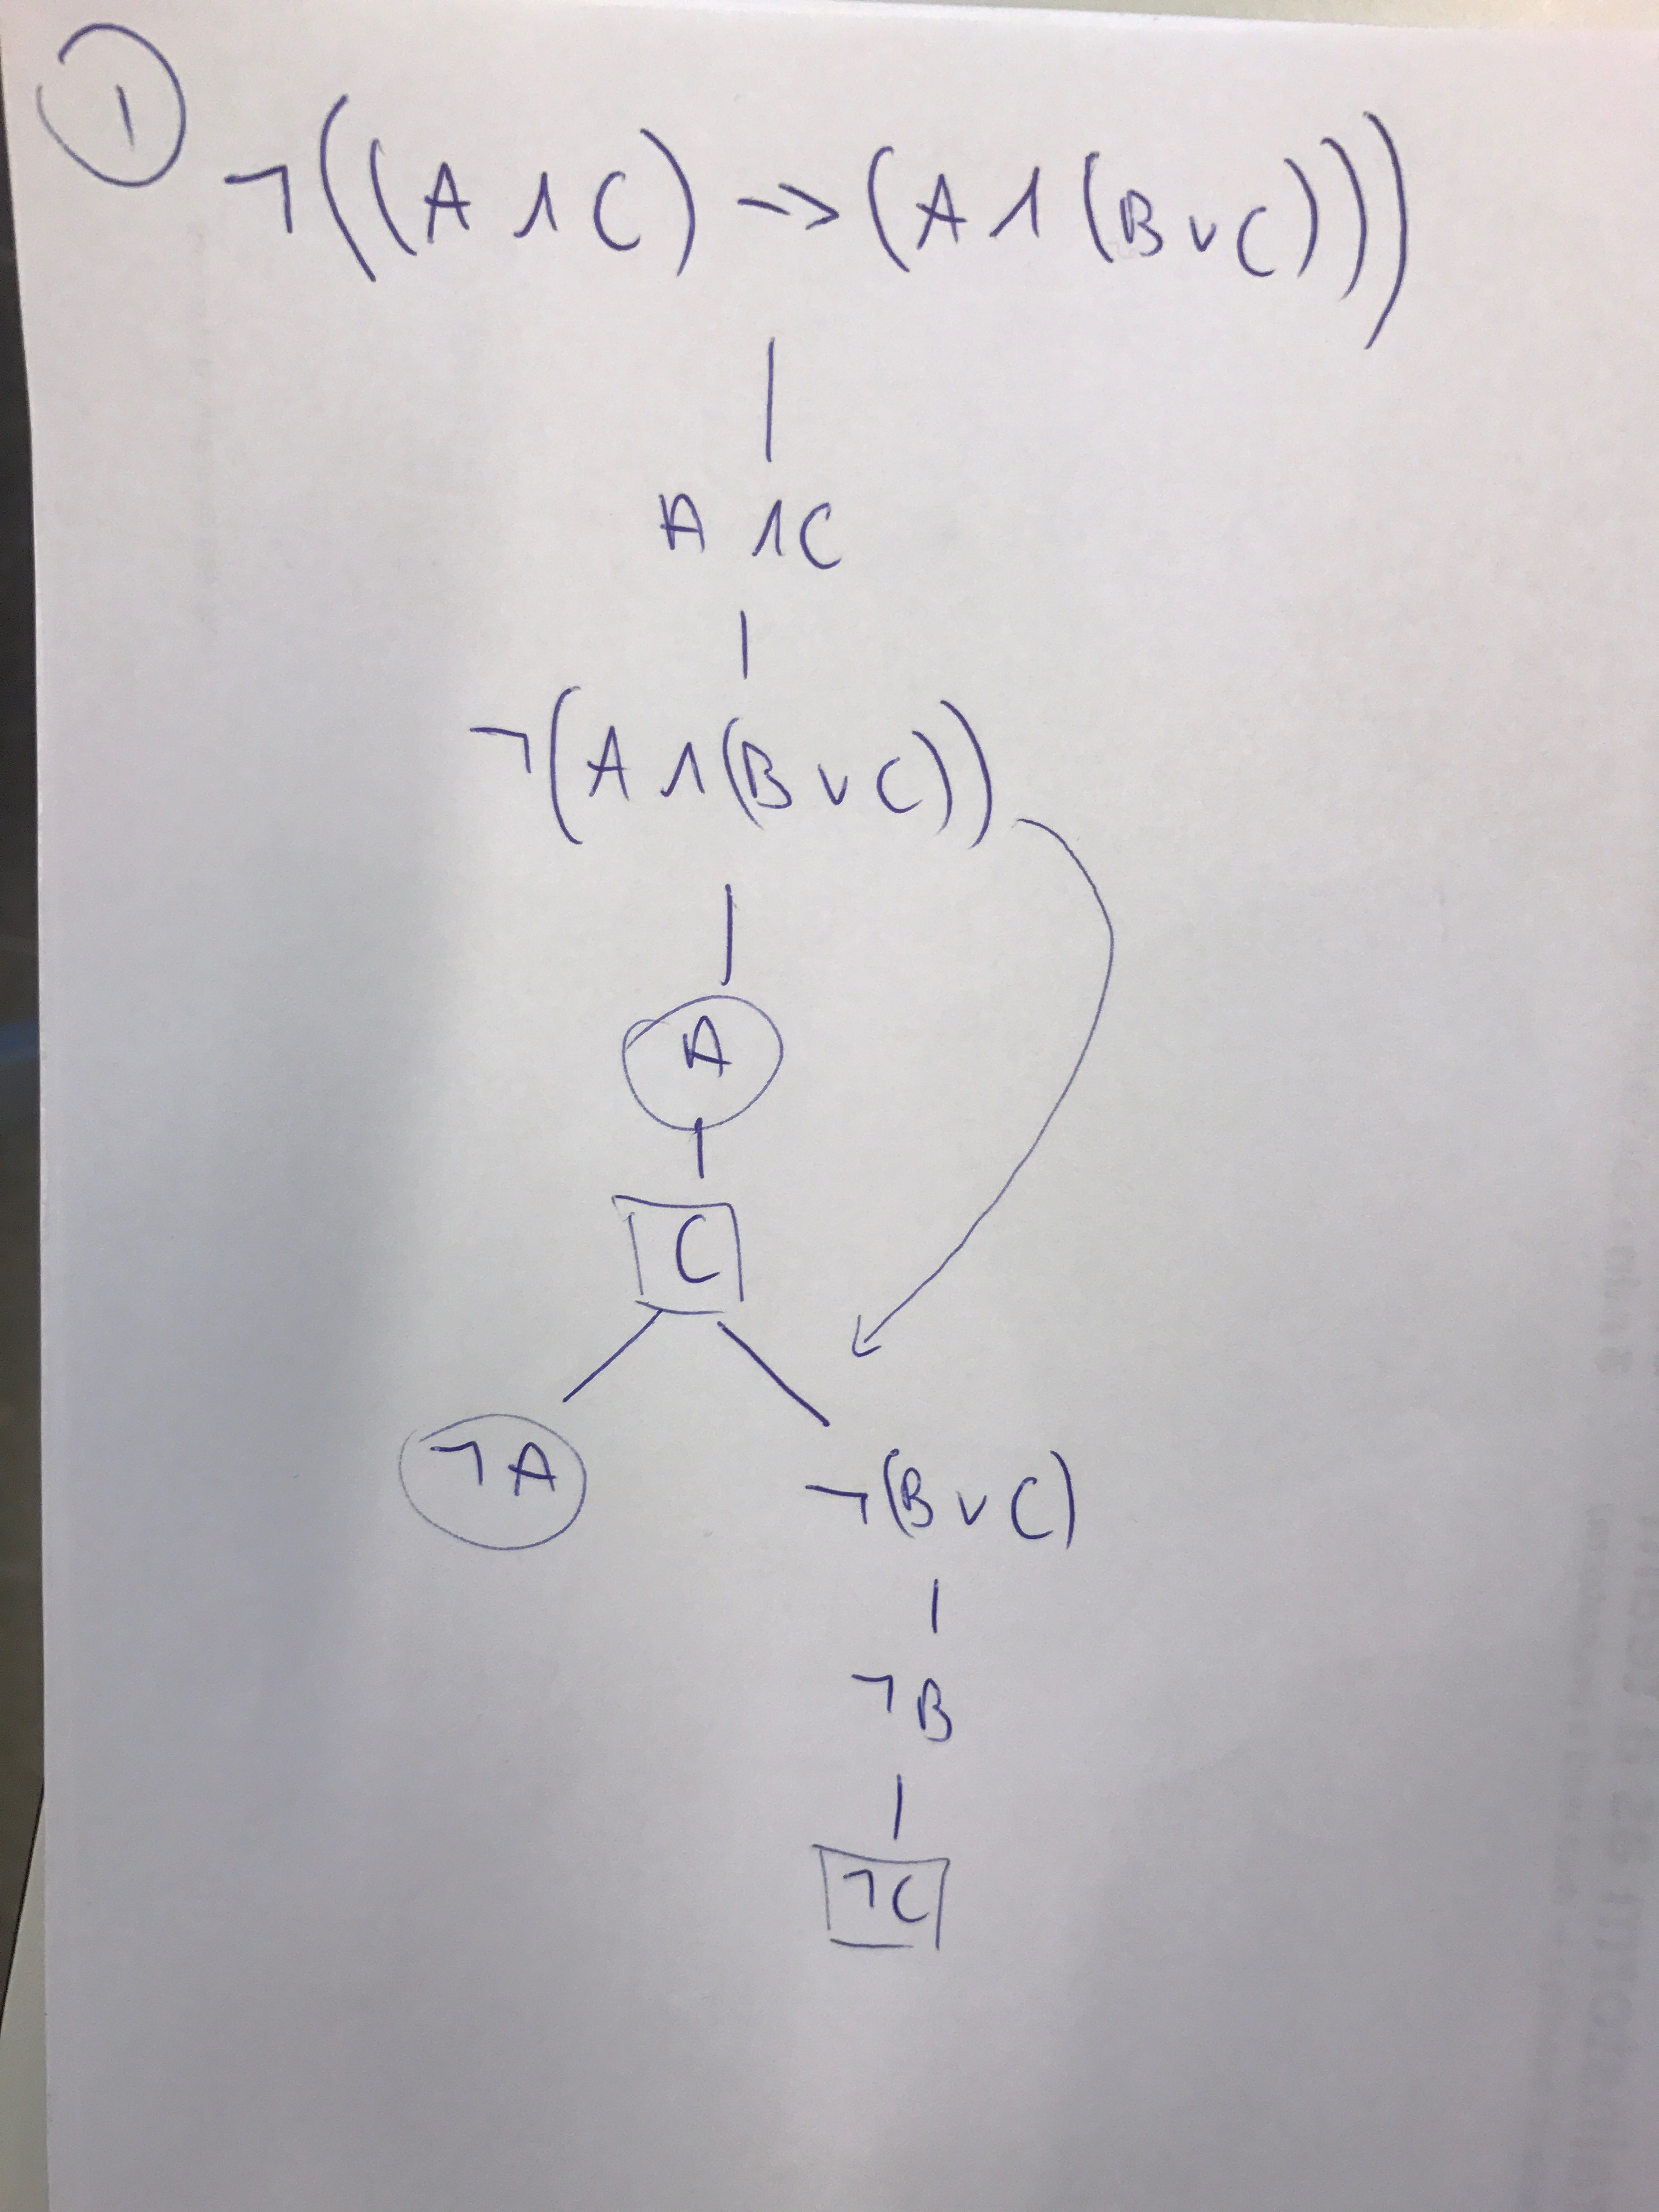
\includegraphics[width=0.5\textwidth]{images/workshop7_problem1.jpg} 
		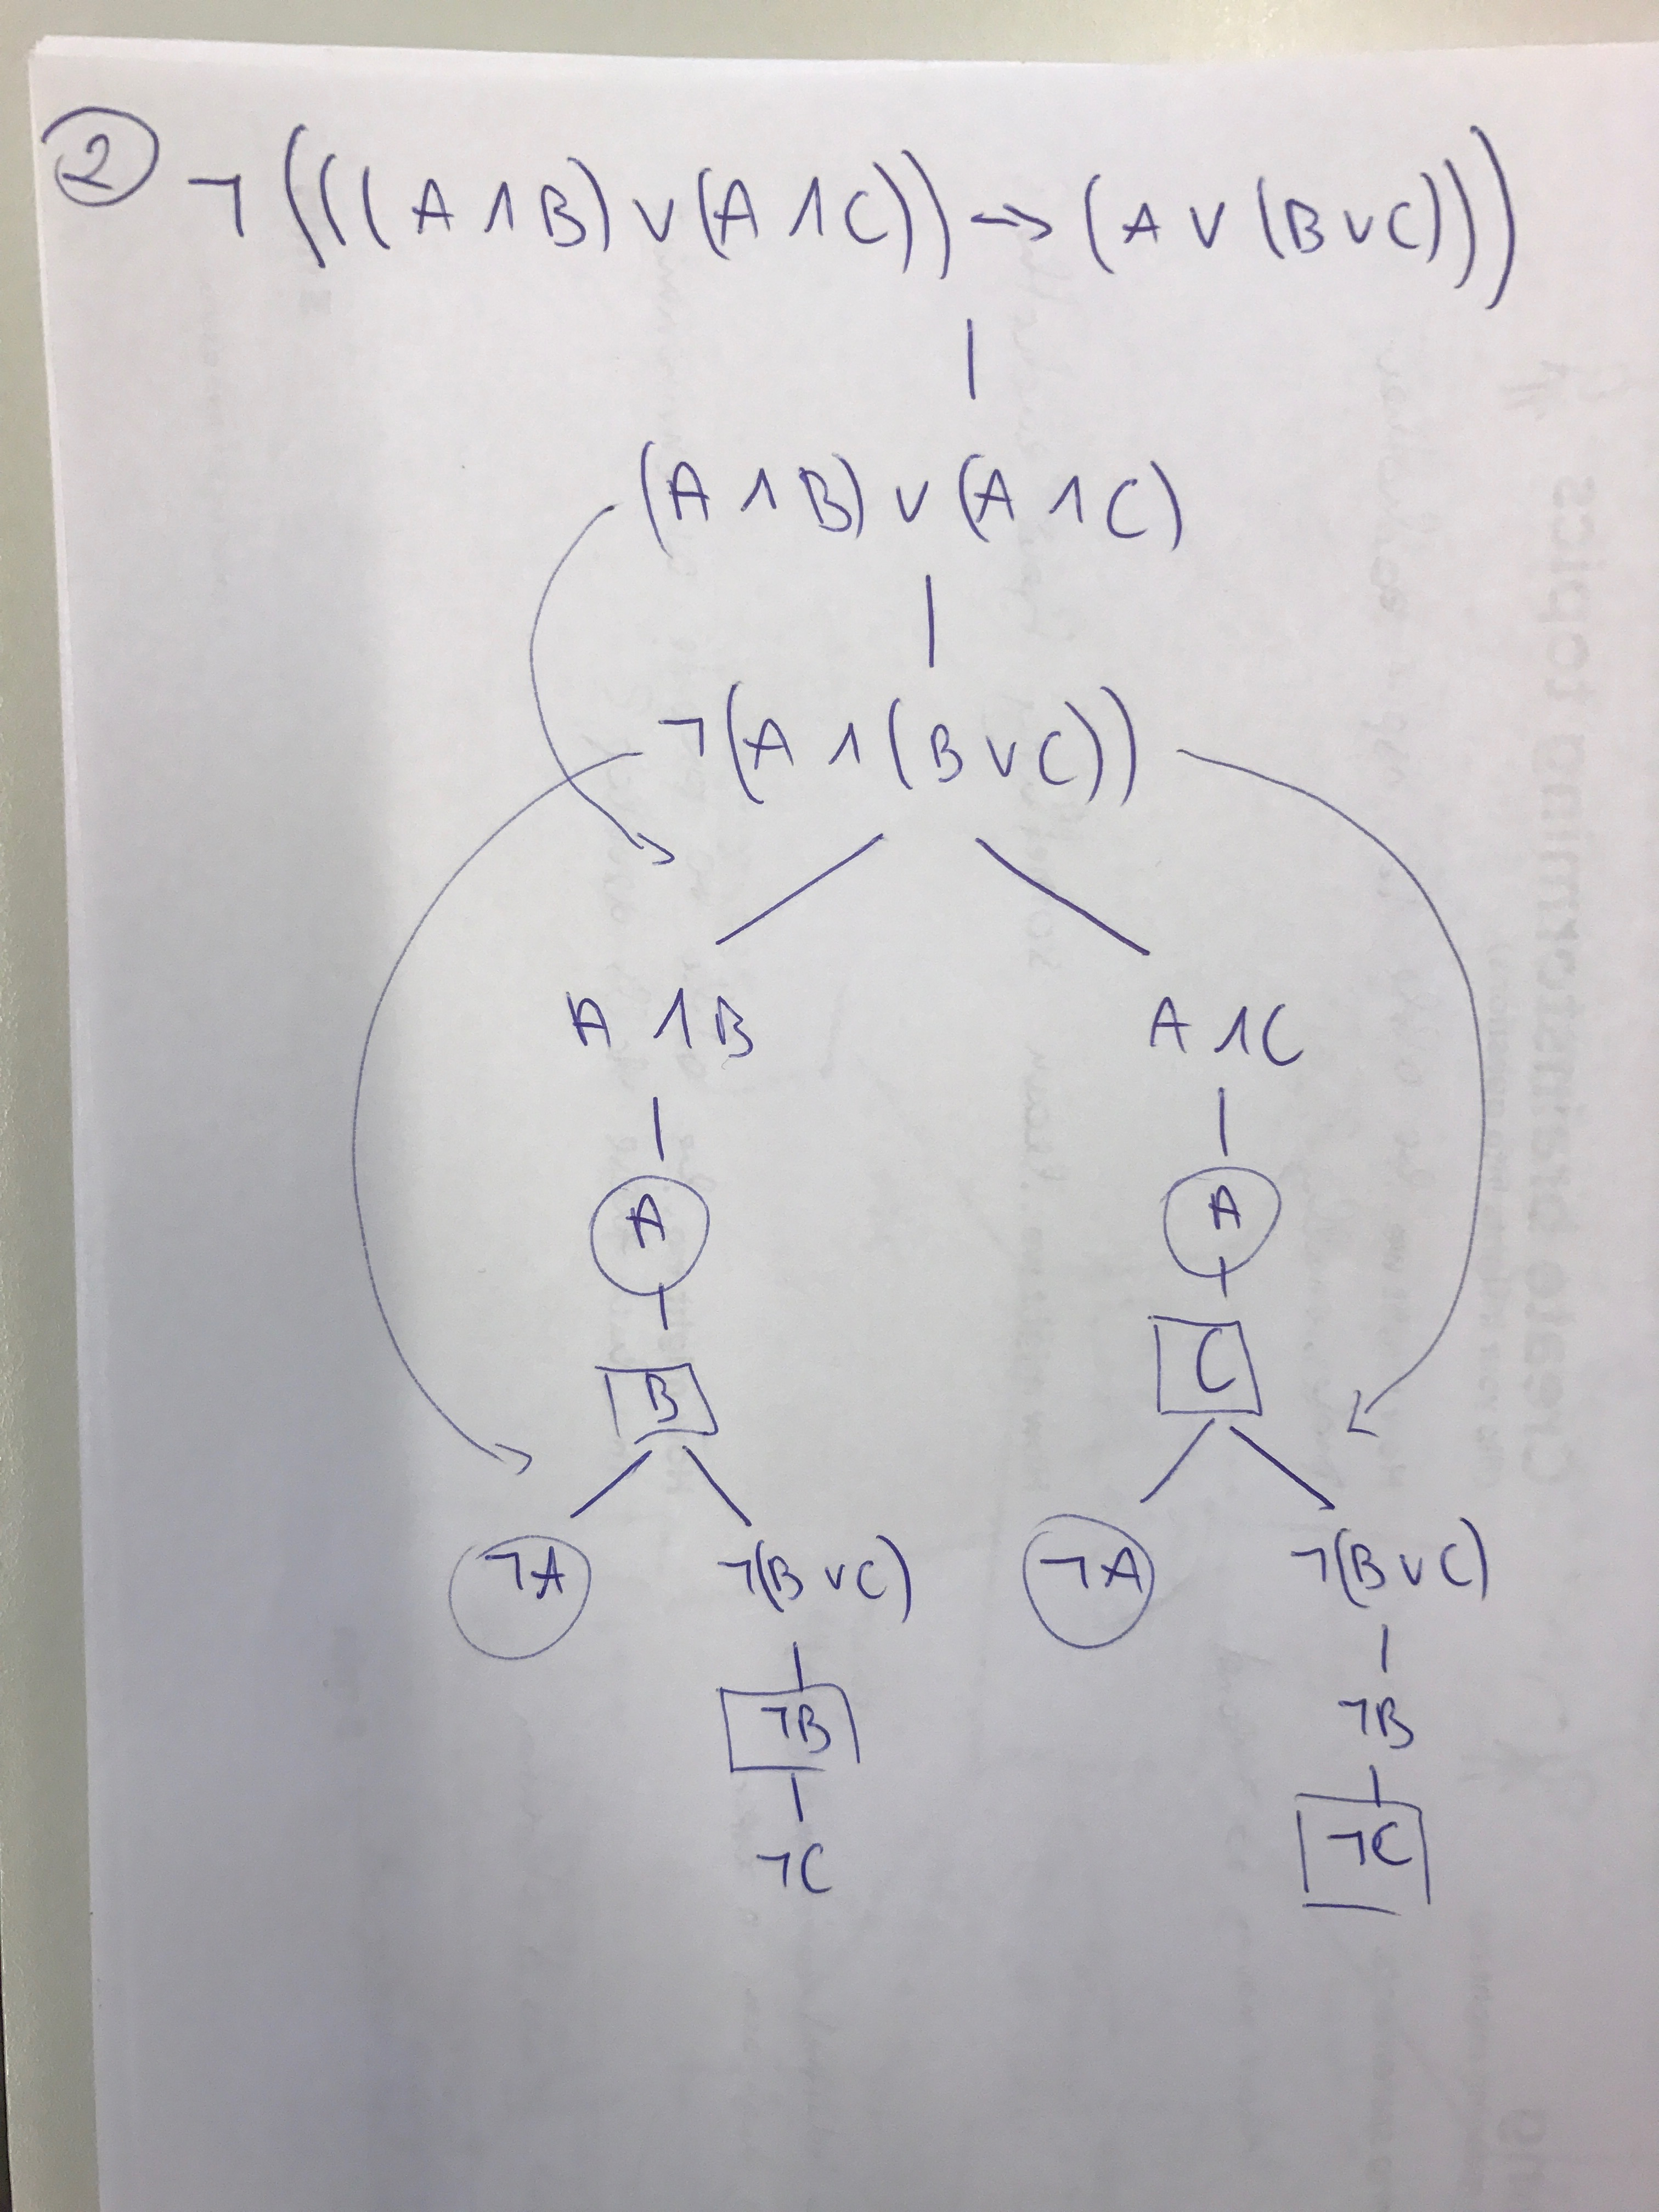
\includegraphics[width=0.5\textwidth]{images/workshop7_problem2.jpg}
		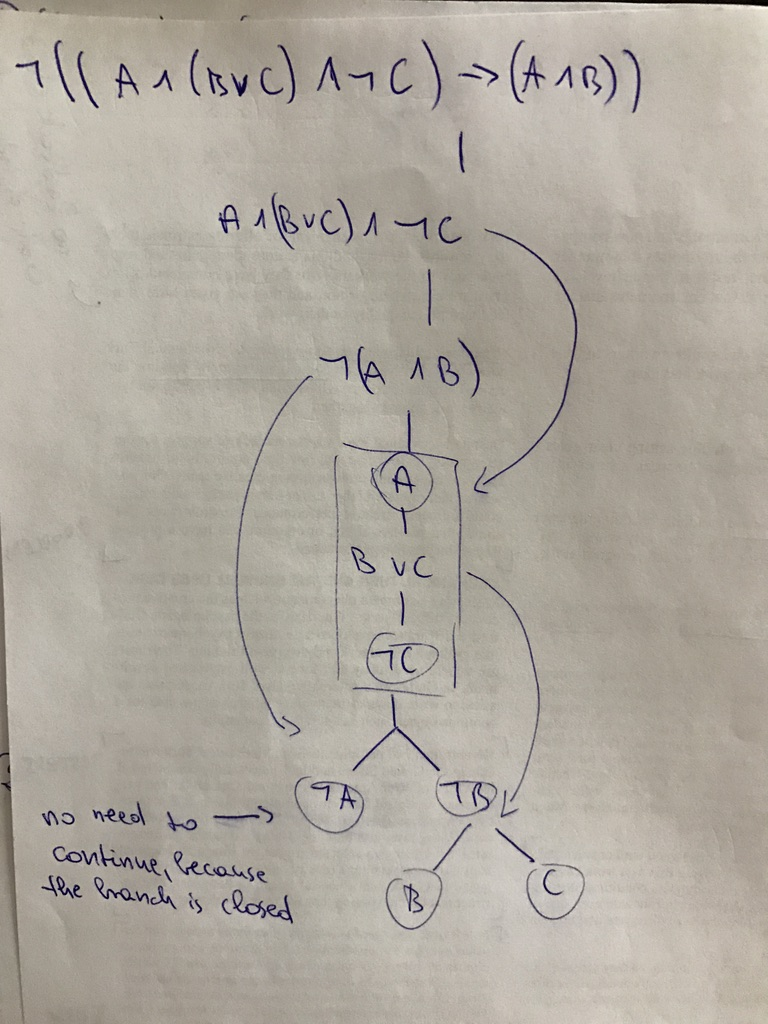
\includegraphics[width=0.5\textwidth]{images/workshop7_problem3.jpg}
		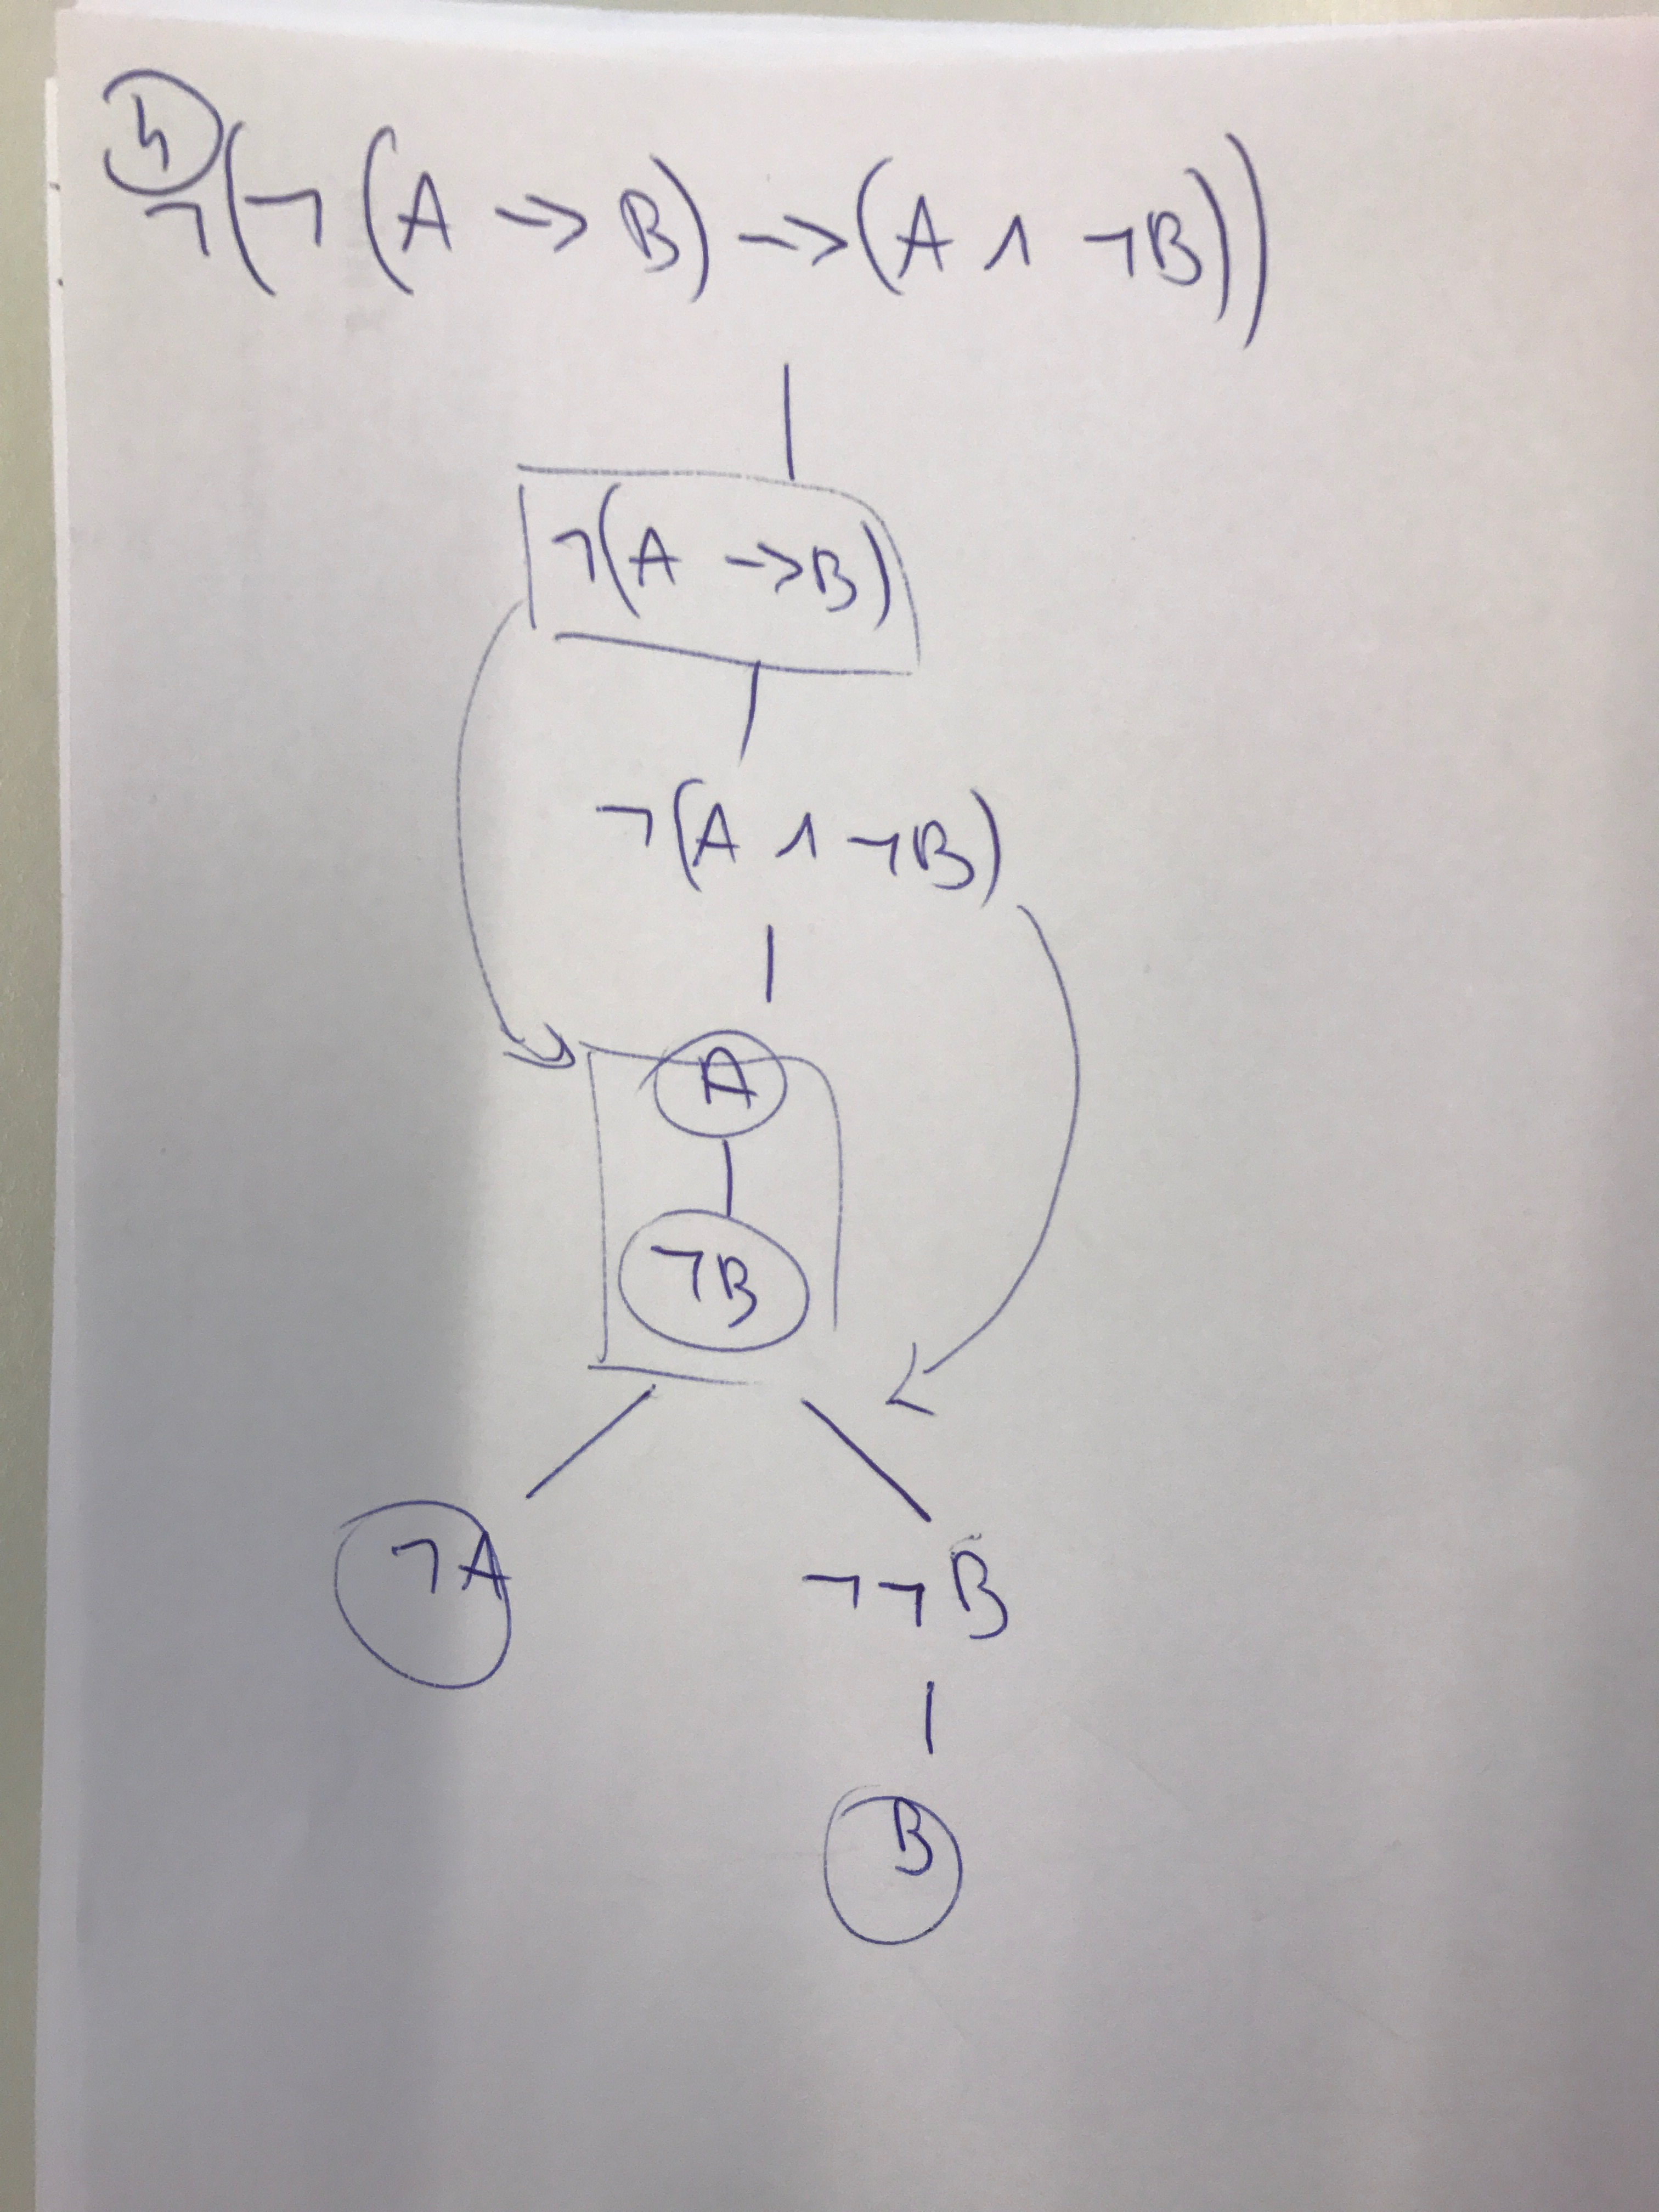
\includegraphics[width=0.5\textwidth]{images/workshop7_problem4.jpg}
	\end{center}
\section{Problem 5}
To express the given formula in DNF and CNF, we us its truth table below and read the corresponding lines to construct both forms. 

\begin{center}
		\begin{tabular}{c|c|c||c|c|c}
		\toprule
		$p_0$ & $p_1$ & $p_2$ & $p_1 \iff p_2$ & $\neg p_0 \rightarrow (p_1 \vee p_2)$ & $(p_1 \iff p_2 ) \wedge (\neg p_0 \rightarrow (p_1 \vee p_2))$ \\ 
		\midrule
		0 & 0 &  0 & 1 & 0 & 0 \\
		0 & 0 &  1 & 1 & 1 & 1 \\ 
		0 & 1 &  0 & 0 & 1 & 0 \\
		0 & 1 &  1 & 0 & 1 & 0 \\ 
		1 & 0 &  0 & 0 & 1 & 0 \\
		1 & 0 &  1 & 0 & 1 & 0 \\
		1 & 1 &  0 & 1 & 1 & 1 \\		
		1 & 1 &  1 & 1 & 1 & 1 
		\end{tabular}
		\end{center}
	
	DNF: $(\neg p_0 \wedge \neg p_1 \wedge p_2) \vee (p_1 \wedge p_2 \wedge \neg p_2) \vee (p_1 \wedge p_2 \wedge p_2)$	
	
	CNF: $(p_0 \vee p_1 \vee p_2) \wedge (p_0 \vee \neg p_1 \vee p_2) \wedge (p_0 \vee \neg p_1 \vee \neg p_2) \wedge (\neg p_0 \vee p_1 \vee p_2) \wedge (\neg p_0 \vee p_1 \vee \neg p_2)$
	
\section{Problem 6}
To show that $\{\vee, \rightarrow \}$ is not a universal set of connectives, we explain why the $\wedge$ or the $\neg$ functions cannot be expressed in terms of the operators in the set. It is easy to see that the $\neg$ function can be expressed with the function $p \rightarrow p$ as shown in the truth table below. 

\begin{center}
\begin{tabular}{c||c||c}
\toprule
$p$ & $\neg p$ & $p \rightarrow p$ \\ 
\midrule
0 & 1 & 1 \\
1 & 0 & 0
\end{tabular}
\end{center}

Therefore, we should find a reasoning why the $\wedge$ connective is not possible to be defined with the operators $\{\vee, \rightarrow \}$. We should observe that the $\wedge$ function always gives 1 as an output only if both input values are 1 and yields in 0 otherwise. Similarly, the $\vee$ function yields in 1 if at least one of the inputs is 1 and the $\rightarrow$ function yields in 0 if and only if the first input value is 0 and the second is 1. 

Because of these properties, there is no way to apply the $\vee, \rightarrow$ connectives in any way on the input values to satisfy the requirements of the $\wedge$ connective.

\section{Problem 7}
To evaluate the given propositional, we take a look at its truth table below. 

	\begin{center}
		\begin{tabular}{c|c|c||c}
		\toprule
		$p_0$ & $p_1$ & $p_2$ & $((p_0 \rightarrow p_1) \rightarrow p_2) \rightarrow p_0$ \\
		\midrule
		0 & 0 &  0 & 1 \\
		0 & 0 &  1 & 0 \\ 
		0 & 1 &  0 & 1 \\
		0 & 1 &  1 & 0 \\ 
		1 & 0 &  0 & 1 \\
		1 & 0 &  1 & 1 \\
		1 & 1 &  0 & 1 \\		
		1 & 1 &  1 & 1
		\end{tabular}
	\end{center}
	
	We can see that the truth value of the function is 1 under some valuation and 0 under another valuation. Therefore, the formula is contingent.

\section{Problem 8}
\end{document}